 \begin{figure}[H]
\centering
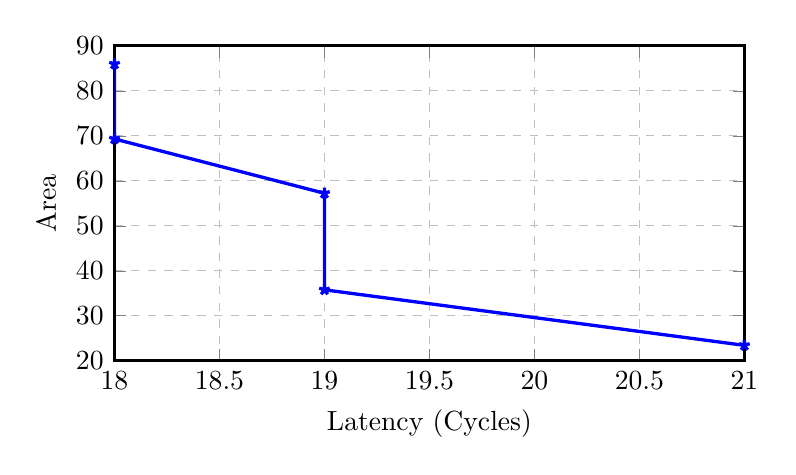
\begin{tikzpicture}
\begin{axis}[
scale only axis,
height=4cm,
width=8cm,
    xlabel={Latency (Cycles)},
    ylabel={Area},
    xmin=18, xmax=21,
    ymin=20, ymax=90,
    xtick={18,18.5,19,19.5,20,20.5,21},
    ytick={20,30,40,50,60,70,80,90},
    legend pos=north east,
    ymajorgrids=true,
    xmajorgrids=true,
    grid style=dashed,
    very thick
]
\addplot[
    color=blue,
    mark=star,
    %smooth
    ]
    coordinates {
    (18,85.95)(18,69.3)(19,57.225)(19,35.77)(21,23.429)
    };
\end{axis}
\end{tikzpicture}
\caption{Area Vs. Latency Curve for Butterfly Unit Implementation}
\label{plot_butterfly}
\end{figure}